\section{Zusammenfassung und Ausblick}

\begin{figure}
	\centering
	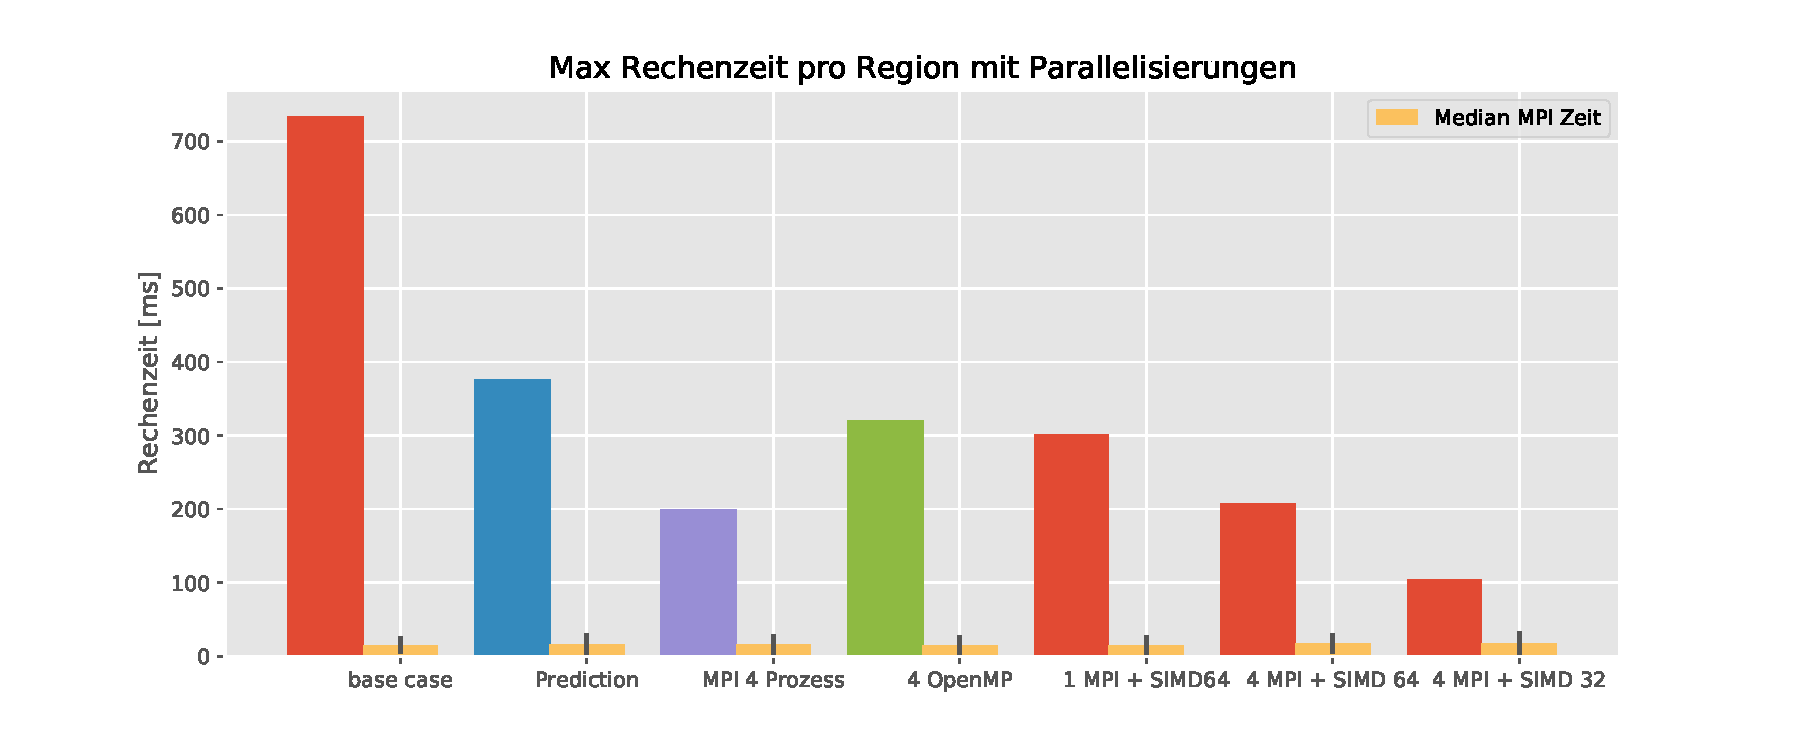
\includegraphics[width=0.9\linewidth]{img/Zusammenfassung/overall}
	\caption{Kombination der unterschiedlichen Parallelisierungsstrategien.
		Es wurden für jede der Konfigurationen \( 3 \) Regionen am Rand mit \( 40 \) Konten evaluiert.}
	\label{fig:overallScaling}
\end{figure}

Abschließend lassen sich noch die unterschiedlichen, in den vorheringen Abschnitten erläuterten,
Strategien zur Parallelisierung der Berechnung der Mandelbrotmenge miteinander kombinieren. Dadurch
kann die maximal erzielbare Verringerung der Rechenzeiten evaluiert werden, welche in \autoref{fig:overallScaling}\footnote{\enquote{Speedup} bezieht sich dabei auf
	die Maximale Rechenzeit für die Berechnung der 3 Randregionen mit 40 Knoten \( (723 ms) \)}
dargestellt sind.

\begin{figure}[h!]
	\centering
	\begin{tabular}{lc}
		Konfiguration                             & Speedup    \\
		\hline
		Naive Balancierung                        & \( 1 \)    \\
		Lastbalancierung mit Vorhersage           & \( 1.95 \) \\
		4 MPI Prozesse pro Knoten                 & \( 3.69 \) \\
		4 OpenMP Prozesse pro Knoten              & \( 2.29 \) \\
		1 MPI Prozess pro Konten mit SIMD 64 bit  & \( 2.43 \) \\
		4 MPI Prozesse pro Konten mit SIMD 64 bit & \( 3.54 \) \\
		4 MPI Prozesse pro Konten mit SIMD 32 bit & \( 7.05 \) \\
	\end{tabular}
\end{figure}

Somit ergibt sich, dass wir unter der Verwendung aller implementierten Parallelisierungen eine Verbesserung
der maximalen Rechenzeit im Vergleich zu einer naiven Lastbalancierung vom Faktor \( \approx 7 \) erzielen konnten,
was einer absoluten Rechenzeit von \( 104ms \) für \( 1280px \times 720px \) große Ausschnitte am Rand der Mandelbrotmenge erzielen konnten.

\pagebreak
Ziel des Projektes war es, ein Programm zur parallelen Berechnung der Mandelbrotmenge auf einem Rechnercluster zu erstellen.
Dazu wurden drei unterschiedliche Ansätze der Parallelisierung genutzt:
\begin{itemize}
	\item \textbf{MPI:} Verteilung der Rechenlast auf die Hardwareknoten des Clusters, Kommunikation über Nachrichten zwischen den Knoten
	\item \textbf{OpenMP:} Verteilung der Rechenlast auf die CPU-Kerne eines Knotens, Kommunikation über geteilten Speicher
	\item \textbf{SIMD:} Verteilung der Rechenlast innerhalb eines CPU-Kernes durch Nutzung von Vektorregistern
\end{itemize}

Die Verteilung auf verschiedene Rechenknoten erfordert eine Lastbalancierung, damit die Knoten gleichmäßig ausgelastet werden.
Hier wurden dafür zwei verschiedene Strategien realisiert:
\begin{itemize}
	\item \textbf{Naive Strategie:} Aufteilung in gleich große Bereiche
	\item \textbf{Strategie mit Vorhersage:} Aufteilung in Bereiche mit gleichem Rechenaufwand mithilfe einer Heuristik
\end{itemize}

Weiterhin sollte der Effekt der Parallelisierung für den Nutzer deutlich werden.
Dazu gibt es eine Web-Schnittstelle in der die Mandelbrotmenge optisch ansprechend dargestellt wird und von der Nutzerin erkundet werden kann.

%%%%%%
% Ausblick
%   automatische bestimmung der optimalen knotenmenge
%   erweiterung der fraktale/balancer zwecks didaktik allg. stärkerer HDI/Didaktik interaktion fokus
\paragraph{Ausblick}
Als eine Weiterführung dieses Projekts könnten andere Fraktale,
wie zum Beispiel Julia-Mengen betrachtet werden.
Auch komplexere Fraktale, zum Beispiel Buddhabrot, stellen eine interessante Herausforderung dar. Sowie weitere Fraktale,
bei denen nicht alle Pixel unabhängig von einander berechnet werden können.
Weiterhin könnte eine dynamische Variante der Lastbalancierung mit sogenanntem \textit{Job-Stealing} realisiert werden.
Zusätzlich könnte die Webschnitstelle in so fern erweitert werden, als das noch mehr
Parameter der Berechnung, wie Anzahl an Knoten oder maximale Iterationszahl, durch die Endbenutzerin einstellbar sind.